%\iffalse
\let\negmedspace\undefined
\let\negthickspace\undefined
\documentclass[journal,12pt,twocolumn]{IEEEtran}
\usepackage{cite}
\usepackage{amsmath,amssymb,amsfonts,amsthm}
\usepackage{algorithmic}
\usepackage{textcomp}
\usepackage{xcolor}
\usepackage{txfonts}
\usepackage{listings}
\usepackage{enumitem}
\usepackage{mathtools}
\usepackage{gensymb}
\usepackage{comment}
\usepackage[breaklinks=true]{hyperref}
\usepackage{tkz-euclide} 
\usepackage{listings}
\usepackage{gvv}                            \usepackage{tikz}
\usepackage{circuitikz}
\def\inputGnumericTable{}                                
\usepackage[latin1]{inputenc}                            
\usepackage{color}                                       
\usepackage{array}                                       
\usepackage{longtable}                                   
\usepackage{calc}                              
\usepackage{tikz}
\usepackage{multirow}                                    
\usepackage{hhline}                                      
\usepackage{ifthen}                            
\usepackage{caption}
\usepackage{lscape}
\usepackage{amsmath}
\newtheorem{theorem}{Theorem}[section]
\newtheorem{problem}{Problem}
\newtheorem{proposition}{Proposition}[section]
\newtheorem{lemma}{Lemma}[section]
\newtheorem{corollary}[theorem]{Corollary}
\newtheorem{example}{Example}[section]
\newtheorem{definition}[problem]{Definition}
\newcommand{\BEQA}{\begin{eqnarray}}
\newcommand{\EEQA}{\end{eqnarray}}
\newcommand{\define}{\stackrel{\triangle}{=}}
\theoremstyle{remark}
\newtheorem{rem}{Remark}

\begin{document}

\bibliographystyle{IEEEtran}
\vspace{3cm}

\title{GATE 2021 EE.20}
\author{EE23BTECH11010 - VENKATESH BANDAWAR$^{*}$% <-this % stops a space
}
\maketitle
\newpage
\bigskip

\section{Laplace Transform}
Laplace transform of integrals:\\
Let the function defined as $y(t) = \int_0^t f(u) du$ for all $t > 0$\\
Laplace transform of y(t) in t 
\begin{align}
    \mathcal{L} \brak{y(t)} &= \int_0^{\infty} e^{-st} y(t) dt\\
    &= \int_0^{\infty} e^{-st} \int_0^t f(u) du dt\\
    &= \int_0^t f(u) du \sbrak{- \frac{e^{-st}}{s}}_0^{\infty} + \int_0^{\infty} \frac{e^{-st}}{s} f(t) dt\\
    &= \frac{F(s)}{s}
\end{align}


\section{RLC Low Pass Filter}
\begin{figure}[!ht]
    \centering
    \begin{circuitikz}
   \draw(0,0) to [R](2,0);
   % \draw (2,0) -- (2.5,0);
   \draw(2,0) to [L] (4,0);
   % \draw (5,0) to (5,0);
   \draw (4,0) to [C] (4,-2);
   \draw(4,-2)  to (0,-2);
   \draw (4,0) -- (5,0);
   \draw (4,-2)to (5,-2);
   \node[circle,fill,inner sep=1pt] at (0,0) {};
   \node[circle,fill,inner sep=1pt] at (5,0) {};
   \node[circle,fill,inner sep=1pt] at (5,-2) {};
   \node[circle,fill,inner sep=1pt] at (0,-2) {};
   \draw[->](0,-1.85) to (0,-0.15);
   \draw[->](5,-1.85) to (5,-0.15);
   \node at (0.3,-1) {$x(t)$};
   \node at (5.5,-1) {$y(t)$};

   \node at (1,0.5) {$R$};
   \node at (3,0.5) {$L$};
   \node at (2.8,-1) {$C$};\node[circle,fill,inner sep=1pt] at (0,0) {};
\end{circuitikz}

    \caption{RLC Low pass filter}
\end{figure}
\begin{table}[!ht]
    \centering
    \begin{tabular}{|c|c|c|}
\hline
    Parameter & Description & Value\\
    \hline
    $P(s)$ & Plant Transfer Function & $\frac{0.001}{s\brak{\frac{s}{0.5}+1}\brak{\frac{s}{100}+1}}$\\
    \hline
    $C(s)$ & Lag Compensator  & $\frac{100\brak{\frac{s}{10}+1}}{\frac{s}{0.1}+1}$\\
    \hline
    $T(s)$ & Loop gain  & $P(s) C(s)$ \\
    \hline
    $\omega$ & Angular Frequency & 3rad/s \\
    \hline
\end{tabular}

    \caption{Input Parameters}
\end{table}
\begin{align}
    Y(s) &= I(s)Z_C\\
    &= \frac{X(s)}{Z_L + Z_R + Z_C}Z_C\\
    H(s) &= \frac{Y(s)}{X(s)}\\
    &= \frac{Z_C}{Z_L + Z_R + Z_C}\\
    &= \frac{\frac{1}{sC}}{sL + R + \frac{1}{sC}}\\
    &= \frac{1}{s^2LC + sRC + 1}\\
    \implies H(s) &= \omega_0^2\frac{1}{(s-p_1)(s-p_2)}
\end{align}
where,
\begin{align}
    \omega_0 &= \frac{1}{\sqrt{LC}}\\
    p_{1, 2} &= -\frac{R}{2L} \pm \sqrt{\brak{\frac{R}{2L}}^2 - \frac{1}{LC}}\\
    &= -\alpha \pm \sqrt{\alpha^2 - \omega_0^2}
\end{align}
where
\begin{align}
    \alpha &= \frac{R}{2L}
\end{align}
Damping Factor is given by,
\begin{align}
   \zeta &= \frac{\alpha}{\omega_0}\\
   &= \frac{R}{2}\sqrt{\frac{C}{L}}
\end{align}
\begin{table}[!ht]
    \centering
    \begin{tabular}{|c|c|c|c|}
\hline
\textbf{Parameter}&\textbf{Description} &\textbf{subquestion}& \textbf{Value}\\
\hline
     \multirow{4}{*}{$\Delta \theta$} & \multirow{4}{*}{$\theta_1 - \theta_2$} &\brak{a}& 6.4$\pi$ \, radians \\
     \cline{3-4}
     & & \brak{b}& 0.8$\pi$ \, radians \\
     \cline{3-4}
     & &\brak{c}& $\pi$ \, radians \\
     \cline{3-4}
     & & \brak{d} & $\dfrac{3\pi}{2\vphantom{\brak{0.1}}}$ \, radians \\
     \hline
\end{tabular}

    \caption{Effect of Damping Coefficient $\zeta$ on system behaviour}
\end{table}
\newpage
\begin{enumerate}
\item Overdamped Response
\begin{align}
    Y(s) &= X(s)H(s)\\
    &= \omega_0^2\frac{1}{s(s-p_1)(s-p_2)}\\
    &= \frac{c_0}{s} + \frac{c_1}{s-p_1} + \frac{c_2}{s-p_2}
\end{align}
where,
\begin{align}
    c_0 &= 1\\
    c_1 &= \frac{p_2}{p_1 - p_2}\\
    c_2 &= \frac{p_1}{p_2 - p_1}
\end{align}
Taking inverse Laplace,
\begin{align}
    y(t) &= c_0 + c_1e^{p_1t} + c_2e^{p_2t}\\
    &= \brak{1 + \frac{p_2}{p_1 - p_2}e^{p_1t} +  \frac{p_1}{p_2 - p_1}e^{p_2t}}u(t)
\end{align}

\begin{figure}[!ht]
    \centering
    \begin{tikzpicture}
      \draw[<->] (-4,0) -- (1,0) node[right] {$\mathcal{R}(s)$};
    \draw[<->] (0,-2) -- (0,2) node[above] {$\mathcal{I}(s)$};
     \node[orange, cross out, draw, thick, inner sep=2pt] at (-2,0) {};
  \node[orange, cross out, draw, thick, inner sep=2pt] at (-3,0) {};
  \node at (-3,-0.4) {\small $P_1$};
  \node at (-2,-0.4) {\small $P_2$};
\end{tikzpicture}

    \caption{s-Plane for Overdamped case}
\end{figure}

\item Critically Damped Response
\begin{align}
    Y(s)&=X(s)H(s)\\
    &= \omega_0^2\frac{1}{s(s-p)^2}\\
    &= \frac{c_0}{s}+\frac{c_1}{\left(s-p\right)^2}+\frac{c_2}{s-p}
\end{align}
where
\begin{align}
    c_0 &= 1\\
    c_1 &= p\\
    c_2 &= -1
\end{align}
Taking Inverse Laplace,
\begin{align}
    y(t) &= c_0+(c_1t+c_2)e^{pt}\\
    &= \brak{1+(pt-1)e^{pt}}u(t)
\end{align}
\begin{figure}[!ht]
    \centering
    \begin{tikzpicture}
      \draw[<->] (-4,0) -- (1,0) node[right] {$\mathcal{R}(s)$};
    \draw[<->] (0,-2) -- (0,2) node[above] {$\mathcal{I}(s)$};
     \node[orange, cross out, draw, thick, inner sep=2pt] at (-2,0) {};
  % \node at (-3,-0.4) {\small $P_1$};
  \node at (-2,-0.4) {\small $P_{1,2}$};
\end{tikzpicture}

    \caption{s-Plane for Critically damped case}
\end{figure}

\item Underdamped Response
\begin{align}
    Y(s) &= X(s)H(s)\\
    &= \omega_0^2\frac{1}{s(s-p)(s-p^\ast)}\\
    &= \frac{c_0}{s}+\frac{c_1}{s-p}+\frac{c_2}{s-p^\ast}
\end{align}
where,
\begin{align}
    c_0 &= 1\\
    c_1 &= \frac{p^\ast}{p-p^\ast}\\
    c_2 &= \frac{p}{p^\ast-p}
\end{align}
Taking Inverse Laplace,
\begin{align}
    y(t) &= c_0+c_1e^{pt}+c_2e^{p^\ast t}\\
    &= 1+\frac{\abs{p}}{\omega_d}\ e^{-\sigma t}\frac{
    e^{j(\omega_d t+\varphi)}+e^{-j(\omega_d t+\varphi)}}{2}\\
    &= \brak{1+\frac{|p|}{\omega_d}e^{-\sigma t}\cos(\omega_d t+\varphi)}u(t)
\end{align}
where,
\begin{align}
    \abs{p}&=\sqrt{{\omega_d}^2+\sigma^2}\\
    \omega_d&=\omega_0\sqrt{1-\zeta^2}\\
    \sigma&=\omega_0\zeta\\
    \varphi&=\pi-\tan^{-1}\frac{\sigma}{\omega_d}
\end{align}
\begin{figure}[!ht]
    \centering
    \begin{tikzpicture}
    \draw[<->] (-4,0) -- (2,0) node[right] {$\mathcal{R}(s)$};
    \draw[<->] (0,-3) -- (0,3) node[above] {$\mathcal{I}(s)$};
       % \draw[blue, thick, ->] (-2,1) -- (0,2);
       %  \draw[blue, thick, ->] (-2,-1) -- (0,2);

  \draw [blue,arrows = {-Latex[width=0pt 10, length=10pt]}] (-2,1) -- (0,2);
   \draw [blue,arrows = {-Latex[width=0pt 10, length=10pt]}] (-2,-1) -- (0,2);

   \draw[brown, dashed] (-2,1) -- (0,1);
   \draw[brown, dashed] (-2,1) -- (-2,-1);
   \draw[brown, dashed] (-2,-1) -- (0,-1);
   \draw[red, dashed] (-2,1) -- (0,0);

   \node at (-2.2,1) {\small$P_{_1}$};
   \node at (-2.2,-1) {\small$P^*$};
   \node [orange]at (-1.7,0.2) {\small$-\sigma$};
   \node[blue] at (0.3,2) {\small $j\omega$};
    \node[brown] at (0.5,1) {\small $j\omega_d$};
    \node[brown] at (0.5,-1) {\small $-j\omega_d$};
    \node[red] at (-1.45,0.6){\small $\omega_0$};
    % \draw[dashed,->] (0,0.25) ++(-0.222:0.111) arc (90:153.5:0.25);
    \draw[brown,dashed,<->] (0,0.5) arc (90:153.5:0.5);
    \node [purple]at (-0.45,0.65) {\tiny$\sin^{-1}\zeta$};
\end{tikzpicture}

    \caption{s-Plane for Under damped case}
\end{figure}
\end{enumerate}
\begin{figure}
    \centering
    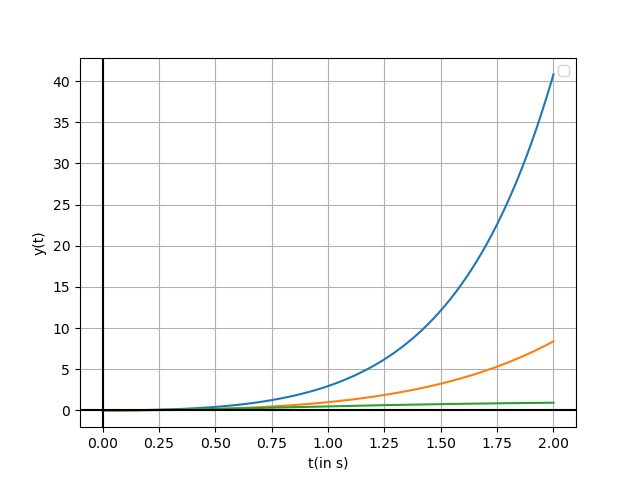
\includegraphics[width = \columnwidth]{figs/plot.png}
    \caption{Plot of y(t) in all three cases}
\end{figure}
\end{document}
